\documentclass[8pt,a4paper]{article}
\usepackage{graphicx}
\usepackage{amsmath}
\usepackage{amsfonts}
\usepackage{setspace}
\usepackage{amssymb,amsthm,epsfig,epstopdf,titling,url,array}
\theoremstyle{plain}
\newtheorem{thm}{Theorem}[section]
\newtheorem{lem}[thm]{Lemma}
\newtheorem{prop}[thm]{Proposition}
\newtheorem*{cor}{Corollary}

\theoremstyle{definition}
\newtheorem{defn}{Definition}[section]
\newtheorem{conj}{Conjecture}[section]
\newtheorem{exmp}{Example}[section]

\theoremstyle{remark}
\newtheorem*{rem}{Remark}
\newtheorem*{note}{Note}
\onehalfspace
\providecommand{\abs}[1]{\lvert#1\rvert}
\providecommand{\norm}[1]{\lVert#1\rVert}
\begin{document}
\title{Reproducing Kernel Hilbert Spaces(RKHS)}
\author{Roberto Alcover Couso}
\date{29/9/2018}
\begin{titlepage}
\maketitle
\end{titlepage}
\section{Introduction}
In this document we will study a special type of Hilbert spaces, RKHS, with a kernel which meets the reproducing property. Understanding this is key for our study due to it's relevance in statistical models and the ideas behind algorithims such as RDC,HSIC...
Furthermore we will define a homogeneity test based on embeddings of probability distributions on RKHSs, where the distance between distributions corresponds to the distance between their embeddings. We will see that the unit ball of an RKHS is a rich enough space so that the expression for the discrepancy vanishes only if the two probability distributions are equal. At the same time it is restrictive enough for the empirical estimate at the discrepancy to converge quickly to its population counterpart as the sample size increases.
\subsection{Preliminar knowledge}

\begin{enumerate}
\item \textsf{Feature map}: $\phi$ is known as a feature map if is a function which maps the data to a Hilbert space $\mathcal{H}$ (feature space).

\begin{align*}
\phi : \mathcal{X} \rightarrow \mathcal{H} \\
x \mapsto \varphi
\end{align*}
\item \textsf{Kernel function}:
k is called a kernel function if it is the dot product defined on a feature space.

Then, we can rewrite the dot product of the space in terms of this mapping:

$$
k: \mathcal{X}\times\mathcal{X} \rightarrow \mathcal{H} \\
(x,x') \mapsto k(x,x')= <\phi(x),\phi(x') >$$
\item \textsf{Reproducing kernel}:
a function k is a reproducing kernel of the Hilbert space $\mathcal{H}$ is and only if it satisfies:
\begin{enumerate}
\item k(x,.)$\in \mathcal{H}, \forall x \in \mathcal{X}$
\item \textit{Reproducing property}: $<f,k(x,\cdot)> = f(x) \forall f \in \mathcal{H} , \forall x \in \mathcal{X}$
\end{enumerate}
\end{enumerate}
\begin{prop}
If k is a reproducting kernel then: $k(x,x') = <k(x,\cdot),k(x',\cdot)>$
\end{prop}
\section{Maximum mean discrepancy}
In this section it'll be shown how RKHSs can be used to define a homogeneity test in terms of the embeddings of the probability measures.
This test consist in maximizing the measure of discrepancy between functions that belong to a certain family $\mathcal{F}$ which must be rich enough to detect all the possible differences between the two probability measures.
\subsection{Mean embedding}

\begin{lem}
Given two Borel probability measures $\mathbb{P}$ and $\mathbb{Q}$  are equal if and only if $\mathbb{E}f(X) = \mathbb{E}f(Y)$  $\forall f \in \mathcal{C(X)}$

$$X \sim \mathbb{P} \text{ and } Y \sim \mathbb{Q}$$
\end{lem}
\begin{flushleft}
This condition is pretty dificult to prove therefore we will keep our study in order to simplify this evaluation.
\end{flushleft}

\begin{defn}\textsf{\textbf{MMD}}

Let $\mathcal{F}$ be a class of functions f: $X \rightarrow \mathbb{R}$ the MMD based on $\mathcal{F}$ is

\end{defn}
\begin{center}
$\gamma(\mathbb{P},\mathbb{Q}) = MMD(\mathcal{F},\mathbb{P},\mathbb{Q}) =  \sup\limits_{f\in\mathcal{F}}\{\mathbb{E}f(X) -\mathbb{E}f(Y)\}$
\end{center}
\begin{flushleft}
This $\mathcal{F}$ must be rich enough for it to ensure that $\mathbb{P} = \mathbb{Q} \leftrightarrow \gamma(\mathbb{P},\mathbb{Q}) = 0$. And restrictive enough for the empirical estimate to converge quickly as the sample size increases.
This will be done through RKHS with a characteristic kernel K
\end{flushleft}
\begin{defn}
\textsf{\textbf{Riesz representation}}
\begin{flushleft}
If T is a bounded linear operator on a Hilbert space $\mathcal{H}$, then there exist some $g \in \mathcal{H}$ such that $\forall f \in \mathcal{H}$:
\end{flushleft}
\begin{center}
$T(f) = <f,g>_{\mathcal{H}}$
\end{center}
\end{defn}

\begin{lem}
Given a K(s,) semi positive definite, measurable and $\mathbb{E}\sqrt{k(X,X)}<\infty$, where X$\sim \mathbb{P}$ then $\mu_{p} \in \mathcal{H}$ exist and fulfulls the next condition
$\mathbb{E}f(X) = <f,\mu_{p}>$ for all f $\in \mathcal{H}$
\end{lem}
\begin{proof}

Lets define the linear operator $T_{\mathbb{P}}f\equiv\mathbb{E}(\sqrt{k(X,X)}) < \infty \forall f\in \mathcal{H}$ 

$$|T_{\mathbb{P}}f| = |\mathbb{E}(f(X))| \leq \mathbb{E}(|f(X)|) =\footnote{Reproducing property of the kernel} \mathbb{E}\abs{<f,k(\cdot,X)>_{\mathcal{H}}} \leq\footnote{Chauchy Schwarz inequality} \norm{f} _{\mathcal{H}}\cdot\mathbb{E}(\sqrt{K(X,X)})^{1/2} <\footnote{The expectation under $\mathbb{P}$ of the kernel is bounded} \infty $$



Then using the Riesz representation theorem applied to $T_{p}$, there exist a $\mu_{p}\in \mathcal{H}$ such that $T_{p}f = <f,\mu_{p}>_{\mathcal{H}}$
\end{proof} 

\begin{defn}
\textsf{\textbf{Mean embedding}}

Given a probability distribution $\mathbb{P}$ we will define the mean embedding of $\mathbb{P}$ as an element $\mu_{p} \in \mathcal{H}$ such that

$$\mathbb{E}(f(X))=<f,\mu_{\mathbb{P}}>_{\mathcal{H}}, \forall f \in \mathcal{H}$$

If $f\in \mathcal{H}$ and $\mu_{\mathbb{P}} \in \mathbb{R}$
$\mathbb{E}(f(X)) = \lim\limits_{N \to \infty} \frac{1}{N} \sum\limits_{n=1}^{N}f(x_{n})$

Applying the Riesz representation theorem to represent $f(x_{n})$

$\forall x_{n}$ then:

$$f(x_{n}) = <f,K(\cdot,x_{n})>_{\mathcal{H}}$$


then

$$\lim\limits_{N \to \infty} \frac{1}{N} \sum\limits_{n=1}^{N}f(x_{n}) = \lim\limits_{N \to \infty} \frac{1}{N} \sum\limits_{n=1}^{N} <f,K(\cdot,x_{n}>_{\mathcal{H}} = <f, \lim\limits_{N \to \infty} \frac{1}{N} \sum\limits_{n=1}^{N}K(\cdot,x_{n})>_{\mathcal{H}}$$

which leads to the final conclussion:

$\mu_{\mathbb{P}} \equiv \mathbb{E}_{X\sim \mathbb{P}}(K(t,X))$  $t \in [0,T]$
\end{defn}
\textsc{Second interpretation of the mean embedding}

$$\mu_{\mathbb{P}} = \mathbb{E}(K(\cdot,X))$$


\subsection{Introduction to MMD}
\begin{lem}
Given the conditions of Lemma 2.2 ($\mu_{\mathbb{P}} \text{and} \mu_{\mathbb{Q}}$ exist) then:

$X \sim \mathbb{P} \mu_{\mathbb{P}} \equiv \mathbb{E}_{X\sim \mathbb{P}}(K(\cdot,X))$ $Y \sim \mathbb{Q} \mu_{\mathbb{Q}} \equiv \mathbb{E}_{Y\sim \mathbb{Q}}(K(\cdot,Y))$

and:

$$MMD(\mathcal{F},\mathbb{P}, \mathbb{Q}) = \norm{\mu_{\mathbb{P}} - \mu_{\mathbb{Q}}}_{\mathcal{H}}$$
\end{lem}
\begin{proof}
\begin{equation}
\begin{split}
MMD 
& \equiv \sup\limits_{f\in \mathcal{H} \norm{f} \leq 1}\{\mathbb{E}(f(x)) - \mathbb{E}(f(y))\} \\
& =\sup\limits_{f\in \mathcal{H}  \norm{f} \leq 1}\{<f,\mu_\mathbb{P}> - <f, \mu_\mathbb{Q}> \} \\
& =\sup\limits_{f\in \mathcal{H} \norm{f} \leq 1} <f,(\mu_{\mathbb{P}} - \mu_{\mathbb{Q}})> \\
& \leq\footnote{ Cauchy Schwarz inequality} \sup\limits_{f\in \mathcal{H} \norm{f}  \leq 1} \{\norm{f}_{\mathcal{H}},\norm{\mu_\mathbb{P} - \mu_{\mathbb{Q}}}_{\mathcal{H}}\} \\
& \leq \norm{\mu_{\mathbb{P}} - \mu_{\mathbb{Q}}}_{\mathcal{H}}.
\end{split}
\end{equation}

But on the other side, if we choose f as:

$$f=\frac{1}{\norm{\mu_{\mathbb{P}}- \mu_{\mathbb{Q}}}} (\mu_{\mathbb{P}}- \mu_{\mathbb{Q}})$$

then we have:

$$\sup\limits_{f\in \mathcal{H} \\\ \norm{f} \leq 1}\{\norm{f}_{\mathcal{H}},\norm{\mu_\mathbb{P} - \mu_{\mathbb{Q}}}_{\mathcal{H}}\} \geq \norm{\mu_{\mathbb{P}}- \mu_{\mathbb{Q}}}_{\mathcal{H}} $$

therefore

$$MMD = \norm{\mu_{\mathbb{P}}- \mu_{\mathbb{Q}}}_{\mathcal{H}}$$
\end{proof}
\begin{prop}
Given:
$X,X' \sim \mathbb{P} \text{ and } Y,Y' \sim \mathbb{Q}$ and X and Y are independent then:
$$MMD^{2}(\mathcal{F},\mathbb{P},\mathbb{Q}) = \mathbb{E}(K(X,X')) + \mathbb{E}(K(Y,Y')) - 2\mathbb{E}K(X,Y).$$
\end{prop}
\begin{proof}
\begin{equation}
\begin{split}
MMD^{2}(\mathcal{F},\mathbb{P},\mathbb{Q}) 
& = \norm{\mu_{\mathbb{P}}- \mu_{\mathbb{Q}}}_{\mathcal{H}}^{2} \\
& =<\mu_{\mathbb{P}}- \mu_{\mathbb{Q}},\mu_{\mathbb{P}}- \mu_{\mathbb{Q}}>_{\mathcal{H}}\\
&=<\mathbb{E}(K(\cdot,X))-K(\cdot,Y)),\mathbb{E}(K(\cdot,X'))-K(\cdot,Y'))>\\
&=\mathbb{E}(<K(\cdot,X),K(\cdot,X')> + <K(\cdot,Y),K(\cdot,Y')> - 2<K(\cdot,X)K(\cdot,Y)>)\\
&=\footnote{is due to the reproductive property of the kernel.} \mathbb{E}(K(X,X') + K(Y,Y') -2K(X,Y)) \\
&= \mathbb{E}(K(X,X')) + \mathbb{E}(K(Y,Y')) -2\mathbb{E}(K(X,Y))\\
&= \int\int K(s,t) \underbrace{d(\mathbb{P}-\mathbb{Q})(s)}_{SignedMeasure} d(\mathbb{P}-\mathbb{Q})(t)
\end{split}
\end{equation}
\end{proof}
\subsection*{Prooving that MMD defines an homogeneity test}

\begin{defn}
\textsf{\textbf{Characteristic kernel}}

A reproducing kernel k is a characterisctic kernel if the induced $\gamma_{k}$ is a metric.
\end{defn}
\begin{thm}

If X is a compact metric space, k is continuous and $\mathcal{H}$ is dense in $\mathcal{C}$(X) with respect to the supremum norm, then $\mathcal{H}$ is characteristic.
\end{thm}
\begin{proof}


Being characteristic means that 
$MMD(\mathcal{F},\mathbb{P},\mathbb{Q}) = 0 \leftrightarrow \mathbb{P} = \mathbb{Q}$
\begin{flushleft}
$\rightarrow$
\end{flushleft}

By lemma 1 we know that $\mathbb{P}$ and $\mathbb{Q}$  are equal if and only if $\mathbb{E}f(X) = \mathbb{E}f(Y)$  $\forall f \in \mathcal{C(X)}$

Given that $\mathcal{H}$ is dense in $\mathcal{C}$(X) then:
$$\forall \epsilon >0, f\in\mathcal{C}(X), \exists g\in \mathcal{H} : \norm{f-g}_{\infty} < \epsilon$$

\begin{equation}
\begin{split}
\abs{\mathbb{E}(f(X)) - \mathbb{E}(f(Y))}  
& = \abs{\mathbb{E}(f(X)) - \mathbb{E}(g(X)) + \mathbb{E}(g(X)) - \mathbb{E}(g(Y)) +\mathbb{E}(g(Y)) - \mathbb{E}(f(Y))} \\
&\leq \abs{\mathbb{E}(f(X)) - \mathbb{E}(g(X))} + \abs{\mathbb{E}(g(X)) - \mathbb{E}(g(Y))} +\abs{\mathbb{E}(g(Y)) - \mathbb{E}(f(Y))}\\
&= \abs{\mathbb{E}(f(X)) - \mathbb{E}(g(X))} + \abs{<g,\mu_{\mathbb{P}}-\mu_{\mathbb{Q}}>_{\mathcal{H}} } +\abs{\mathbb{E}(g(Y)) - \mathbb{E}(f(Y))} \\
&\leq \mathbb{E}\abs{f(X) - g(X)} + \abs{<g,\mu_{\mathbb{P}}-\mu_{\mathbb{Q}}>_{\mathcal{H}} } +\mathbb{E}\abs{g(Y) - f(Y)} \\ 
&\leq^{1} \norm{f-g}_{\infty}  + \abs{<g,\mu_{\mathbb{P}}-\mu_{\mathbb{Q}}>_{\mathcal{H}} } + \norm{f-g}_{\infty}\\
&\leq \abs{<g,\mu_{\mathbb{P}}-\mu_{\mathbb{Q}}>_{\mathcal{H}} } + 2\epsilon
\end{split}
\end{equation}
By lemma 3 we know that if MMD = 0 then $\mu_{\mathbb{P}} = \mu_{\mathbb{Q}}$. Hence:
$$\abs{\mathbb{E}(f(X)) - \mathbb{E}(f(Y))} \leq 2\epsilon$$

Then by lemma 1 $\mathbb{P}$ and $\mathbb{Q}$  are equal.

\begin{flushleft}
$\leftarrow$
\end{flushleft}
By definition of MMD.
\end{proof}
\subsection{Application to independence test}

From the MMD criterion we will develop an independence criterion which will be conduced by the following idea:
Given $\mathcal{X} \sim \mathbb{P}$ and $\mathcal{Y} \sim \mathbb{Q}$ whose joint distribution is $\mathbb{P}_{\mathcal{XY}}$ then the test of independence between these variables will be determining if $\mathbb{P}_{\mathcal{XY}}$ is equal to the product of the marginals $\mathbb{P}\mathbb{Q}$. Therefore:

$\mathcal{MMD}(\mathcal{F}, \mathbb{P}_{\mathcal{XY}},\mathbb{P}\mathbb{Q}) = 0$ if and only if $\mathcal{X}$ and $\mathcal{Y}$ are independent.
To characterize this independence test we need to introduce a new RKHS, which is a tensor product of the RKHS’s in which the marginal distributions of the random variables are embedded. Let $\mathcal{X}$ and $\mathcal{Y}$ be two topological spaces and let k and l be kernels on these spaces, with respective RKHS $\mathcal{H}$ and $\mathcal{G}$. Let us denote as $\upsilon((x, y), (x' , y ' ))$ a kernel on the product space $\mathcal{X}\times\mathcal{Y}$ with RKHS $\mathcal{H}_{\upsilon}$. This space is known as the tensor product space $\mathcal{H}\times\mathcal{G}$. Tensor product spaces are defined as follows:
\begin{defn}
\textbf{Tensor product}
The tensor product of Hilbert spaces$\mathcal{H}_{1}$ and $\mathcal{H}_{2}$  with inner products $<·, ·>_{1}$ and
$<·, ·>_{2}$ is defined as the completion of the space $\mathcal{H}_{1}\times\mathcal{H}_{2}$  with inner product  $<·, ·>_{1}$ $<·, ·>_{2}$extended
by linearity. The resulting space is also a Hilbert space.
\end{defn}
\begin{lem}
A kernel $\upsilon$ in the tensor product space  $\mathcal{H}\times\mathcal{G}$ can be defined as:
$$\upsilon((x,y),(x',y')) = k(x,x')l(y,y')$$
\end{lem}
\paragraph{Useful definitions for the following content}
$$\mathbb{E}_{\mathcal{X}}f(\mathcal{X}) = \int f(x)d\mathbb{P}(x)$$
$$\mathbb{E}_{\mathcal{Y}}f(\mathcal{Y}) = \int f(y)d\mathbb{Q}(y)$$
$$\mathbb{E}_{\mathcal{X}\mathcal{Y}}f(\mathcal{X}\mathcal{Y}) = \int f(x,y)d\mathbb{P}_{\mathcal{X}\mathcal{Y}}(x,y)$$

Using this notation, the mean embedding of $\mathbb{P}_{\mathcal{X}\mathcal{Y}}$ and $\mathbb{P}\mathbb{Q}$ are:
$$\mu_{\mathbb{P}_{\mathcal{X}\mathcal{Y}}} = \mathbb{E}_{\mathcal{X}\mathcal{Y}}\upsilon((\mathcal{X},\mathcal{Y}),)$$
$$\mu_{\mathbb{P}\mathbb{Q}} = \mathbb{E}_{\mathcal{X}\mathcal{Y}}\upsilon((\mathcal{X},\mathcal{Y}),)$$
In terms of these embeddings:
$$\mathcal{MMD}(\mathcal{F}, \mathbb{P}_{\mathcal{XY}},\mathbb{P}\mathbb{Q}) = \norm{\mathbb{P}_{\mathcal{X}\mathcal{Y}}-\mu_{\mathbb{P}\mathbb{Q}} }_{\mathbb{H}_{\upsilon}}$$

\section{HSIC}

In this section we will give a short overview of the cross-covariance operators between RKHSs and their Hilbert-Schmidt norms which later will be used to define the Hilbert Schmidt Independence Criterion (HSIC).
After we will determine whether the dependence returned via HSIC is statistically significant by studying an hypothesis test with HSIC as its statistic and testing it empirically.
Finally we will prove the ewuivalence of the HSIC test in terms of the Hilbert-Schmidt norm of the cross covariance operator in terms of the MMD between $\mathbb{P}_{\mathcal{X}\mathcal{Y}}$ and $\mathbb{P}\mathbb{Q}$

\subsection{Cross Covariance operator}

\begin{defn}
\textsf{\textbf{Tensor product operator}}

Let $h \in \mathcal{H},g \in \mathcal{G}$. The tensor product operator $h \otimes g: \mathcal{G}\rightarrow\mathcal{H}$ is defined as:
$$(h \otimes g)(f) = <g,f>_{\mathcal{G}}h, \forall f \in \mathcal{G}$$
\end{defn}
\begin{defn}
\textsf{\textbf{Hilbert-Schmidt norm of a linear operator}}

Let $C:\mathcal{G}\rightarrow\mathcal{H}$ be a linear operator between RKHS $\mathbb{G} $ and $\mathcal{H}$ the Hilbert-Schmidt norm of C is defined as:

$$\norm{C} = \sqrt{\sum{<Cv_{j},u_{i}>^{2}_{\mathcal{H}}}}$$
\end{defn}
\begin{defn}
\textsf{\textbf{Cross-Covariance operator}}

The cross-covariance operator associated with $\mathbb{P}_{XY}$ is the linear operator $C_{XY}:\mathcal{G}\rightarrow\mathcal{H}$ defined as:
$$C_{XY} = \mathbb{E}_{XY}[(\phi(X)-\mu_{\mathbb{P}}) \otimes (\psi(Y) -\mu_{\mathbb{Q}})] =\footnote{distributive property of the tensor product} \mathbb{E}_{XY}[\phi(X) \otimes \psi(Y)] - \mu_{\mathbb{P}} \otimes \mu_{\mathbb{Q}} $$

Which is a generalisation of the cross-covariance matrix between random vectors.
\end{defn}
\begin{defn}
\textsf{\textbf{HSIC}}
We define the Hilbert-Schmidt Independence Criterion for $\mathbb{P}_{\mathcal{X}\mathcal{Y}}$ as the squared HS norm of the associated cross-covariance operator:

$$HSIC(\mathbb{P}_{\mathcal{X}\mathcal{Y}},\mathcal{H},\mathcal{G}) = \norm{C_{XY}}^{2}_{\mathcal{HS}}$$
\end{defn}
\begin{lem}

If we denote $X,X'\sim \mathbb{P}$ and $Y,Y'\sim \mathbb{Q}$ then:

$$HSIC(\mathbb{P}_{\mathcal{X}\mathcal{Y}},\mathcal{H},\mathcal{G}) = \mathbb{E}_{xx'yy'}[k(x,x')l(y,y')] + \mathbb{E}_{xx'}[k(x,x')]\mathbb{E}_{yy'}[l(y,y')] -2\mathbb{E}_{xy}[\mathbb{E}_{x'}[k(x,x')]\mathbb{E}_{y'}[l(y,y')]]$$
\end{lem}

\begin{proof}


First we will simplify the notation of $C_{XY}$
$$ C_{XY} = \mathbb{E}_{XY}[\phi(X) \otimes \psi(Y)] - \mu_{\mathbb{P}} \otimes \mu_{\mathbb{Q}} = \bar{C_{XY}} - M_{XY}$$

Using this notation:

\begin{equation}
\begin{split}
\norm{C_{XY}}^{2}_{\mathcal{HS}}
& = <\bar{C}_{XY} - M_{XY},\bar{C}_{X'Y'} - M_{X'Y'}>_{\mathcal{HS}} \\
& = <\bar{C}_{XY},\bar{C}_{X'Y'}>_{\mathcal{HS}}+< M_{XY}, M_{X'Y'}>-2<\bar{C}_{XY}, M_{X'Y'}>_{\mathcal{HS}}
\end{split}
\end{equation}
Now calculating each of this products individually:

\begin{equation}
\begin{split}
<\bar{C}_{XY},\bar{C}_{X'Y'}>_{\mathcal{HS}} 
& = <\mathbb{E}_{XY}[\phi(X) \otimes \psi(Y)],\mathbb{E}_{X'Y'}[\phi(X) \otimes \psi(Y)] >\\
& = \mathbb{E}_{XY}\mathbb{E}_{X'Y'}\norm{\phi(X) \otimes \psi(Y)}^{2} \\
& = \mathbb{E}_{XY}\mathbb{E}_{X'Y'}\norm{\phi(X)}^{2}\norm{\psi(Y)}^{2}\\
& = \mathbb{E}_{XY}\mathbb{E}_{X'Y'}<\phi(X),\phi(X')><\psi(Y),\psi(Y)> \\
& = \mathbb{E}_{XY}\mathbb{E}_{X'Y'} k(X,X')l(Y,Y') \\
\end{split}
\end{equation}
\begin{equation}
\begin{split}
<M_{XY},M_{X'Y'}>_{\mathcal{HS}}
& = <\mu_{\mathbb{P}}\otimes\mu_{\mathbb{Q}},\mu_{\mathbb{P}}\otimes\mu_{\mathbb{Q}}>_{\mathcal{HS}} \\
& = \norm{\mu_{\mathbb{P}}\otimes\mu_{\mathbb{Q}}}^{2}_{\mathcal{HS}} \\
& = \norm{\mu_{\mathbb{P}}}^{2}_{\mathcal{H}}\norm{\mu_{\mathbb{Q}}}^{2}_{\mathcal{G}} \\
& = <\mu_{\mathbb{P}},\mu_{\mathbb{P}}>_{\mathcal{H}}<\mu_{\mathbb{Q}},\mu_{\mathbb{Q}}>_{\mathcal{G}} \\
& = <\mathbb{E}_{X}k(X,\cdot),\mathbb{E}_{X'}k(X',\cdot)>_{\mathcal{H}}<\mathbb{E}_{Y}l(Y,\cdot),\mathbb{E}_{Y'}k(Y',\cdot)>_{\mathcal{G}} \\
& = \mathbb{E}_{X}\mathbb{E}_{X'}\mathbb{E}_{Y}\mathbb{E}_{Y'}<k(X,\cdot),k(X',\cdot)>_{\mathcal{H}}<l(Y,\cdot),l(Y',\cdot)>_{\mathcal{G}} \\
& = \mathbb{E}_{X}\mathbb{E}_{X'}\mathbb{E}_{Y}\mathbb{E}_{Y'}k(X,X')l(Y,Y') \\
\end{split}
\end{equation}

\begin{equation}
\begin{split}
<\bar{C}_{XY},M_{XY}>_{\mathcal{HS}} 
& = <\mathbb{E}_{XY}[\phi(X) \otimes \psi(Y)],\mu_{\mathbb{P}}\otimes\mu_{\mathbb{Q}}>_{\mathcal{HS}} \\
& = <\mathbb{E}_{XY}[\phi(X) \otimes \psi(Y)],\mathbb{E}_{X'}\phi(X')\otimes\mathbb{E}_{Y'}\psi(Y')>_{\mathcal{HS}} \\
& = <\mathbb{E}_{XY}<\mathbb{E}_{X'}<\mathbb{E}_{Y'}<\phi(X) \otimes \psi(Y),\phi(X') \otimes \psi(Y')>_{\mathcal{HS}} \\
& = <\mathbb{E}_{XY}<\mathbb{E}_{X'}<\mathbb{E}_{Y'}<\phi(X),\phi(X')>_{\mathcal{H}}<\psi(Y),\psi(Y')>_{\mathcal{G}} \\
& = <\mathbb{E}_{XY}<\mathbb{E}_{X'}<\mathbb{E}_{Y'}k(X,X')l(Y,Y').
\end{split}
\end{equation}
\end{proof}
\subsection{Statistics}

In the previous subsection we defined the HSIC statistic.
$$HSIC(\mathbb{P}_{\mathcal{X}\mathcal{Y}},\mathcal{H},\mathcal{G}) = \mathbb{E}_{xx'yy'}[k(x,x')l(y,y')] + \mathbb{E}_{xx'}[k(x,x')]\mathbb{E}_{yy'}[l(y,y')] -2\mathbb{E}_{xy}[\mathbb{E}_{x'}[k(x,x')]\mathbb{E}_{y'}[l(y,y')]]$$

In this section we will define the Empirical HSIC.

\begin{defn}
\textsf{\textbf{Empirical HSIC}}

$$HSIC(\mathbb{P}_{\mathcal{X}\mathcal{Y}},\mathcal{H},\mathcal{G}) = (m-1)^{-2}\textbf{tr}KHLH$$

where: $H,K,L \in \mathbb{R}^{m \times m}$, $K_{i,j} = k(x_{i},y_{j})$ , $L_{i,j} = l(x_{i},y_{j})$ and $H_{i,j} = \delta_{i,j} - m^{-1}$
\end{defn}
\begin{thm}
let $\mathbb{E}_{Z}$ denote the expectation taken over m independent copies($x_{i},y_{i}$ drawn from ${P}_{\mathcal{X}\mathcal{Y}}$. Then:
$$HSIC(\mathbb{P}_{\mathcal{X}\mathcal{Y}},\mathcal{H},\mathcal{G}) = \mathbb{E}_{Z}[HSIC(Z,\mathcal{H},\mathcal{G})] + O(m^{-1})$$.
\end{thm}

\begin{proof}

By definition of H we can write:

$$
\textbf{tr}KHLH = \textbf{tr}KL - 2m^{-1}\mathbf{1}^{T}KL\mathbf{1} + m^{-2}\textbf{tr}K\textbf{tr}L
$$

where $\mathbf{1}$ is the vector of all ones.

Now we will expand each of the terms separately and take expectations with respect to Z.

\begin{enumerate}


\item $\mathbb{E}_{Z}[\textbf{tr}KL]$:
$$
\mathbb{E}_{Z}[\sum_{i}K_{ii}L_{ii} + \sum_{(i,j)\in i_{2}^{m}}K_{ij}L{ji}] = O(m) +(m)_{2}\mathbb{E}_{XYX'Y'}[k(X,X')l(Y,Y')]
$$

Normalising terms by $\frac{1}{(m−1)^{2}}$ yields the first term, since $\frac{m(m−1)}{(m−1)^{2}}=1+O(m^{−1})$.

\item $\mathbb{E}_{Z}[\mathbf{1}^{T}KL\mathbf{1}]$:

$$
\mathbb{E}_{Z}[\sum_{i}K_{ii}L_{ii} + \sum_{(i,j)\in i_{2}^{m}}(K_{ii}L{ij} + K_{ij}L{jj})]  + \mathbb{E}_{Z}[\sum_{(i,j,r)\in i_{3}^{m}} K_{ij}L{jr}] $$

$$= O(m^{2}) +(m)_{3}\mathbb{E}_{XY}[\mathbb{E}_{X'}[k(x,x')]\mathbb{E}_{Y'}[l(Y,Y')]]
$$

Again, normalising terms by $\frac{2}{(m−1)^{2}}$ yields the second term. As before we used that  $\frac{m(m−1)}{(m−1)^{2}}=1+O(m−1)$.

\item $\mathbb{E}_{Z}[\textbf{tr}K\textbf{tr}L]$:

$$
O(m^{3}) + \mathbb{E}_{Z}[\sum_{(i,j,q,r)\in i_{4}^{m}} K_{ij}L{qr}] = O(m^{3}) + 
(m)_{4}\mathbb{E}_{XX'}[k(x,x')]\mathbb{E}_{YY'}[l(Y,Y')]
$$

Normalisation by $\frac{1}{(m−1)^{2}}$ takes care of the last term, which completes the proof.
\end{enumerate}

\end{proof}

\begin{thm}
Under the $\mathcal{H}_{0}$ the U-statistic HSIC cirresponding to the V-statistic 
$$ HSIC(Z) = \frac{1}{m^{4}}\sum_{i,j,q,r \in_{4}^{m}} h_{ijqr}$$ 
is degenerate, meaning $\mathbb{E}h=0$. In this case, HSIC(Z) converges in distribution according to \cite{HSICDegenerate}, section 5.5.2
$$mHSIC(Z)\rightarrow \sum_{l=1} \lambda_{l}z_{l}^{2}$$
where $z_{l}\sim \mathcal{N}(0,1)$ i.i.d and $\lambda_{l}$ are the solutions to the eigenvalue problem
$$
\lambda_{l}\psi_{l}(z_{j}) = \int h_{ijqr}\psi_{l}(z_{i})dF_{iqr}
$$
where the integral is over the distribution of variables $z_{i},z_{q}$ and $z_{r}$\cite{HSICdistribution}
\end{thm}


\paragraph*{Approximating the $1-\alpha$ quantile of the null distribution}

A hypothesis test using HSIC(Z)
could be derived from Theorem 3.3 above by computing the $(1 − \alpha)$th quantile of the distribution  $\sum_{l=1} \lambda_{l}z_{l}^{2}$,
where consistency of the test (that is, the convergence to zero of the Type II error for $m \rightarrow \infty$) is
guaranteed by the decay as $m^{-1}$ of the variance of HSIC(Z) under $H_{1}$ . The distribution under $H_{0}$
is complex, however: the question then becomes how to accurately approximate its quantiles.

One approach taken by \cite{HSICdistribution} is by using a Gamma distribution, which as we can see in the figure underneath is quite accurate.

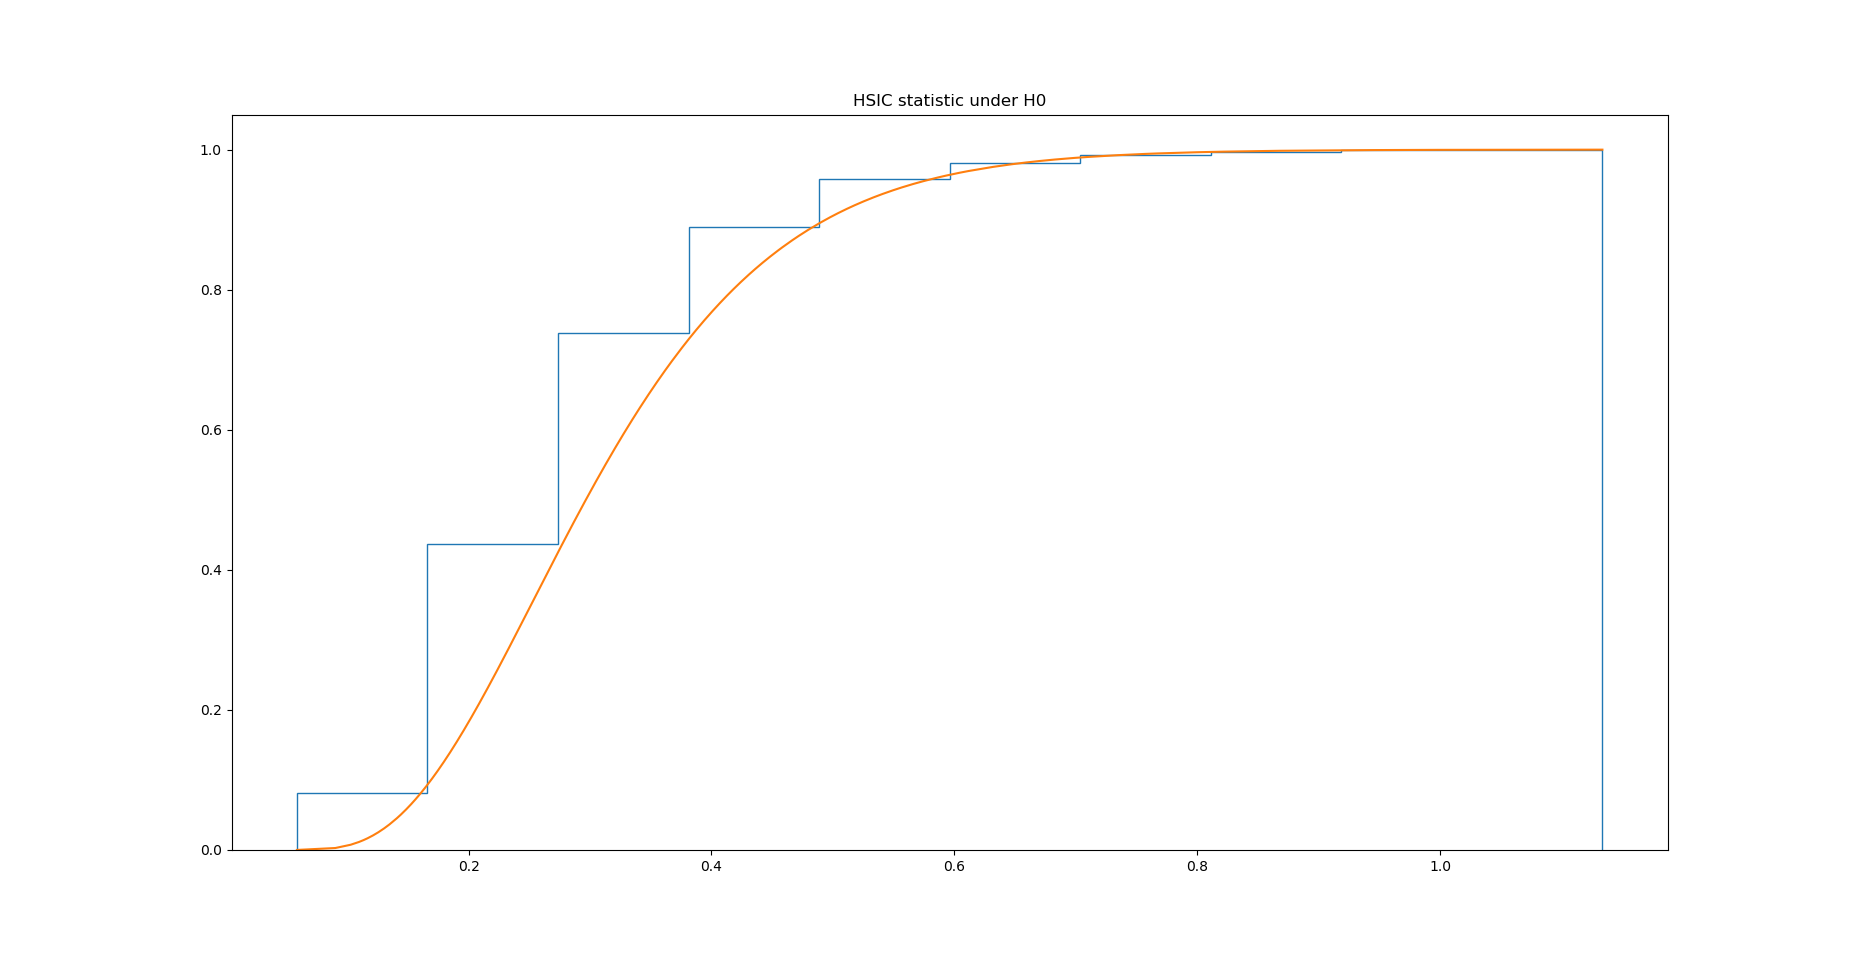
\includegraphics[scale=0.28]{HSIC_DistributionGamma.png}

\section{Energy distance}

In this section we will define energy distance and we will use it to define a homogeneity test.
This knowledge will be used in order to formulate another independence test based on energy distance, distance covariance and distance correlation. This test is one of the most popular nowadays because of its power and the fact that it does not depend on any parameter.

\subsection{Definitions}
One of the simplest distances we can define between two distributions F and G is the L 2 one,
although it has the drawback that the distribution of its natural estimate is not distribution-free.
That is, the distribution of the estimate depends on the distribution F under the null hypothesis.
However, we can extend this distance easily to higher dimensions, having the property of being
rotation invariant. Then energy distances can be derived as a variation of the L 2 distance, given
by the following proposition:
\begin{prop}
Let $\mathcal{F}$ and $\mathcal{G}$ be two CDFs of the independent random variables X,Y respectively and  X',Y' two iid copies of them, then:
$$
2\int_{-\infty}^{\infty}(\mathcal{F}(x) - \mathcal{G}(x))^{2} dx = 2\mathbb{E}\abs{X-Y} - \mathbb{E}\abs{X-X'} -\mathbb{E}\abs{Y-Y'}  
$$
\end{prop}
\begin{proof}
We will start analysing the expectations of the right hand side. We will use that for any positive random variable $ Z>0$,
$\mathbb{E}Z = \int_{0}^{\infty} \mathbb{P}(Z>z)dz$
\begin{equation}
\begin{split}
\mathbb{E}\abs{X-Y}
& = \int_{0}^{\infty} \mathbb{P}(\abs{X-Y} > u) du \\
&= \int_{0}^{\infty} \mathbb{P}(X - Y > u) du + \int_{0}^{\infty} \mathbb{P}(X - Y < u) du \\
&= \int_{0}^{\infty}\int_{-\infty}^{\infty} \mathbb{P}(X - Y > u|Y = y)d\mathcal{G}(y)du + \int_{0}^{\infty}\int_{-\infty}^{\infty} \mathbb{P}(X - Y < u|X = x)d\mathcal{F}(x)(y)du \\
&=\footnote{due to both having finite expectation we can apply fubini}  
\int_{-\infty}^{\infty}\int_{0}^{\infty} \mathbb{P}(X - Y > u|Y = y)du\mathcal{G}(y) + \int_{-\infty}^{\infty}\int_{0}^{\infty} \mathbb{P}(X - Y < u|X = x)du\mathcal{F}(x) \\
&= \int_{-\infty}^{\infty}\int_{0}^{\infty} \mathbb{P}(X > u + y)du\mathcal{G}(y) + \int_{-\infty}^{\infty}\int_{0}^{\infty} \mathbb{P}(Y > u + x)du\mathcal{F}(x)\\
\end{split}
\end{equation}

Now we use the change of variables z = u + y for the first integral, and w = u + x for the second one. Applying Fubini again:

\begin{equation}
\begin{split}
\mathbb{E}\abs{X-Y}
&= \int_{-\infty}^{\infty}\int_{y}^{\infty} \mathbb{P}(X > z)dz\mathcal{G}(y) + \int_{-\infty}^{\infty}\int_{x}^{\infty} \mathbb{P}(Y > w)dw\mathcal{F}(x)\\
&= \int_{-\infty}^{\infty} \mathbb{P}(X > z)dz\int_{y}^{\infty}\mathcal{G}(y) + \int_{-\infty}^{\infty}\mathbb{P}(Y > w)dw\int_{x}^{\infty} \mathcal{F}(x)\\
&= \int_{-\infty}^{\infty} \mathbb{P}(X > z)\mathbb{P}(Y < z)dz + \int_{-\infty}^{\infty}\mathbb{P}(Y > w)\mathbb{P}(X < w)dw\\
&= \int_{-\infty}^{\infty} [(1 - \mathcal{F}(z))\mathcal{G}(z) + (1 - \mathcal{G}(z))\mathcal{F}(z)]dz\\
&= -2\int_{-\infty}^{\infty}\mathcal{F}(z)\mathcal{G}(z)dz + \mathbb{E}\abs{X} + \mathbb{E}\abs{Y}\\
\end{split}
\end{equation}
Taking $\mathcal{F} = \mathcal{G}$ in the previous development:

$$
\mathbb{E}\abs{X-X'} =  -2\int_{-\infty}^{\infty}\mathcal{F}^{2}(z)dz + 2\mathbb{E}\abs{X}
$$

Equivalently for Y. Combining these partial results concludes the proof.

\end{proof}

\begin{thebibliography}{9}
\bibitem{HSICdistribution} Gretton A,Fukumizu K, Teo H.C., Song L, Schölkopf B, Smola J.A.
(2007)
\textit{A Kernel Statistical Test of Independence}
\bibitem{HSICDegenerate} Serfling R.
(Wiley, New York, 1980)
\textit{Approximation Theorems of Mathematical Statistics}

\end{thebibliography}
\end{document}